  \documentclass[a4paper]{article}
  \setlength{\oddsidemargin}{0 in}
  \setlength{\evensidemargin}{0 in}
  \setlength{\topmargin}{-0.6 in}
  \setlength{\textwidth}{6.5 in}
  \setlength{\textheight}{8.5 in}
  \setlength{\headsep}{0.75 in}
  \setlength{\parindent}{0 in}
  \setlength{\parskip}{0.1 in}
  \setlength{\tabcolsep}{0.7pt}
  \usepackage[english]{babel}
  \usepackage[utf8]{inputenc}
  \usepackage{amsmath}
  \usepackage{graphicx}
  \usepackage[colorinlistoftodos]{todonotes}
  \usepackage{algorithm}
  \usepackage{algorithmicx}
  \usepackage{algpseudocode}
  \usepackage{listings}
  \usepackage{color}
  \usepackage{tabularx}
  \usepackage[T1]{fontenc}
  \usepackage{float}

  \definecolor{dkgreen}{rgb}{0,0.6,0}
  \definecolor{gray}{rgb}{0.5,0.5,0.5}
  \definecolor{mauve}{rgb}{0.58,0,0.82}
  \algdef{SE}[DOWHILE]{Do}{doWhile}{\algorithmicdo}[1]{\algorithmicwhile\ #1}%

  \title{Project Proposal: Provisioning applications(platform-as-a-service) using containers}

  \author{Siddhartha Dutta (120040005), Karan Ganju(120050021)}

  \date{\today}

  \begin{document}
  \maketitle

  \section{Problem Description}

  \subsection{Context}
  
  Cloud services are currently divided into the following three categories:
  \begin{enumerate}
	  \item Infrastructure as a service: Takes physical computer hardware such as servers, storage arrays, and networking and lets users build virtual infrastructure that mimics these resources, but which can be created, reconfigured, resized, and removed within moments. Eg. Amazon EC2, S3.
	  \item Platform as a service: Provides a platform allowing customers to develop, run and manage Web applications without the complexity of building and maintaining the infrastructure typically associated with developing and launching an app. Eg. Google App Engine, Heroku, RedHat OpenShift, Cloud Foundary, IBM Bluemix.
	  \item Software as a service: Built on top of a Platform as a Service solution(could be public or private) and provides software for end-users such as email, word processing or a business CRM which could be charged on a per-user or per-month basis. Eg. Adobe Creative Cloud, Office 365.
  \end{enumerate}
  
  PaaS which will be focus of our project is a service required by developers who just want to focus on writing and maintaining their applications without worrying about the infrastructure underneath. They deploy their (usually web) applications on PaaS platforms which take care about providing proper runtime environments and maintaing redundancy, high availability, security and scalability of the applications. Service providers charge customers depending on the guarantees and resources they provide in case its a public service. In private settings quota restrictions can potentially be applied on employees. Cloud virtualization enables developers to be vendor agnostic as they don't need to rely on any particular vendor's API.
  
  PaaS services can be built on top of IaaS or vanilla Linux. One method, when built directly over IaaS whether public(Amazon AWS) or private(OpenStack-based) is to try to run different applications on different VMs. This by its very foundation provides the required isolation. However, its a overkill in terms of resource requirements. Linux has been supporting containers using cgroups even before hardware virtualization based clouds became popular. PaaS services can be provided by making different applications or even different servers of the same application(web, database) run on different containers with all machines running just Linux. This significantly decreases overhead while isolating namespaces but limits flexibility(what about applications that need Windows). 
  
  Apart from the above mentioned dilemma, communication between containers, routing, load balancing, authentication, providing a CLI and GUI interface to users, maintaining a registry of images, dealing with node failure, scheduling and placement of containers/ VMs will be some issues that will be addressed by our project. Security to support multiple tenants and netwrok isolation is required. Not everything needs to be done from scratch. Infact, there are opensource libraries/ frameworks that address the mentioned issues. However, finding, understanding and stitching them together is a non-trivial task in itself.
  
  \subsection{Problem satement}
	
  Building a cloud computing platform as a service(PaaS) enabling developers to deploy applications on demand using containers.
	
  \subsection{Deliverables}

  A front-end(GUI and/ or CLI) for users to:
  \begin{itemize}
	  \item state their CPU, RAM, Storage requirments
	  \item deploy their applications(WAR files) or upload their code(could connect to git)
  \end{itemize}
  
  A front-end(GUI and/ or CLI) for administrators to:
  \begin{itemize}
	  \item see resource usage in various physical machines
	  \item see resource usage by various users
  \end{itemize}
  
  A backend to:
  \begin{itemize}
	  \item measure resource usage of various users
	  \item maintain isolation
	  \item take care of provisioning/ scheduling
	  \item maintain redundancy and availabilty
	  \item authenticate users
	  \item ensure communication between containers of the same user
	  \item maintain security
	  \item manage lifecycles
	  \item balance load
	  \item maintain logs
	  \item check health of applications
  \end{itemize}
  
  Providing runtime environments and frameworks for applications(only a representative subset may be completed depending on the time required for configuration and installation):
	  \begin{itemize}
		  \item Language environments
		  \begin{itemize}
			  \item Java
			  \item Python
			  \item PHP
			  \item Ruby
			  \item Perl
			  \item JavaScript
		  \end{itemize}
		  \item Databases
		  \begin{itemize}
			  \item MongoDB
			  \item MySQL
			  \item PostgreSQL
		  \end{itemize}
		  \item Java-based servers
		  \begin{itemize}
			  \item Apache Tomcat
			  \item JBoss EAP
		  \end{itemize}
		  \item Web application frameworks
		  \begin{itemize}
			  \item Node.js(JavaScript)
			  \item WSGI(Python)
		  \end{itemize}
	  \end{itemize}
	  
  \section{Methodology}
  
  \subsection{Components and Approach Details}
  
  We'll run Ubuntu on a set of machines(depending on how many can be made available). DevStack provides a OpenStack implementation for multiple nodes(OpenStack can be tested online using TryStack). We may use JujuCharms which is a service orchestration management tool. Heat is another orchestration tool. Charms can use Docker to different services in different containers. This will enable us to deploy any service MySQL, PostgrSQL etc. on a container of our choosing. Nagios, Boundary, Tivoli can be used to monitor databases. We may end up modifying and using Cynder for block storage, Swift for object storage, Glance to maintain a repository of images, Keystone for authorization and authentication and Horizon for dashboard management. HAProxy can be used for load balancing while Ceilometer can be used to collect measurements. Kubernetes and Mesos together with Marathon and Zookeeper are also used to manage containers. They can be used with/ without OpenStack. Flannel or Open vSwitch can be used for network management.
  
  We'll need to implement(either from scratch or by using above mentioned tools) the following components:
  
  \begin{enumerate}
	  \item Controller
	  \begin{itemize}
		  \item Orchestrates all other components.
		  \item Performs authentication
		  \item Stores information about the status of other components in the architecture, the users, the deployed applications and available services.
		  \item Exposes a REST interface for accepting requests from the command line tool/ GUI.
		  \item Binds external services like RabbitMQ and MongoDB to the deployed applications.
	  \end{itemize}
	  \item Health Manager
	  \begin{itemize}
		  \item Monitors the health of the deployed applications and other components.
		  \item Corrective actions taken by controller.
		  \item To find out about the health of an application, it compares the current state of a deployed application with the expected state. The expected state of an application that has been running for some time is derived from its initial state. The expected state of an application is available in the controller’s DB.
	  \end{itemize}
	  \item Execution Agent
	  \begin{itemize}
		  \item Component responsible for staging and running all applications.
		  \item Maintains metadata and deploys applications in containers.
		  \item Handles scaling the applications when the load increases by launching new instances of the application.
		  \item Monitors the application that it is running, and generates alerts in case of a change of state.
	  \end{itemize}
	  \item Router
	  \begin{itemize}
		  \item Takes an incoming request, and forwards it to the appropriate container.
		  \item Distributes the load among containers like a load balancer.
		  \item Maintains a routing table which is referred to before making routing decisions.
		  \item If an application that the router sent a request to has failed, the router retries the request with another instance of the same application. 
		  \item The routing table is updated in real time, based on the status of the containers.
	  \end{itemize}
	  \item Messaging
	  \begin{itemize}
		  \item Used by all other components in the architecture for communications.
		  \item Will use asynchronous messaging semantics for high scalability.
		  \item Publish/subscribe messaging called NATS will be used for internal communications.
		  \item Will use RabbitMQ for messaging between applications.
	  \end{itemize}
	  \item Service Abstraction Components
	  \begin{itemize}
		  \item Examples of external services are RabbitMQ, MySQL, mongoDB and Redis. 
		  \item To interface with them, a Service Provisioning Agent can be used. There will be one Service Provisioning Agent for each external service.  
		  \item The Service Gateway is the interface for the Controller to provision external services and to track the status of those services.
		  \item Different services can be tied to each other.
		  \item This module will most likely(I'm yet to explore it completely) make calls to JujuCharms.
	  \end{itemize}
  \end{enumerate}
  
  \subsection{Ordering}
  \begin{figure}[H]
  \centering
  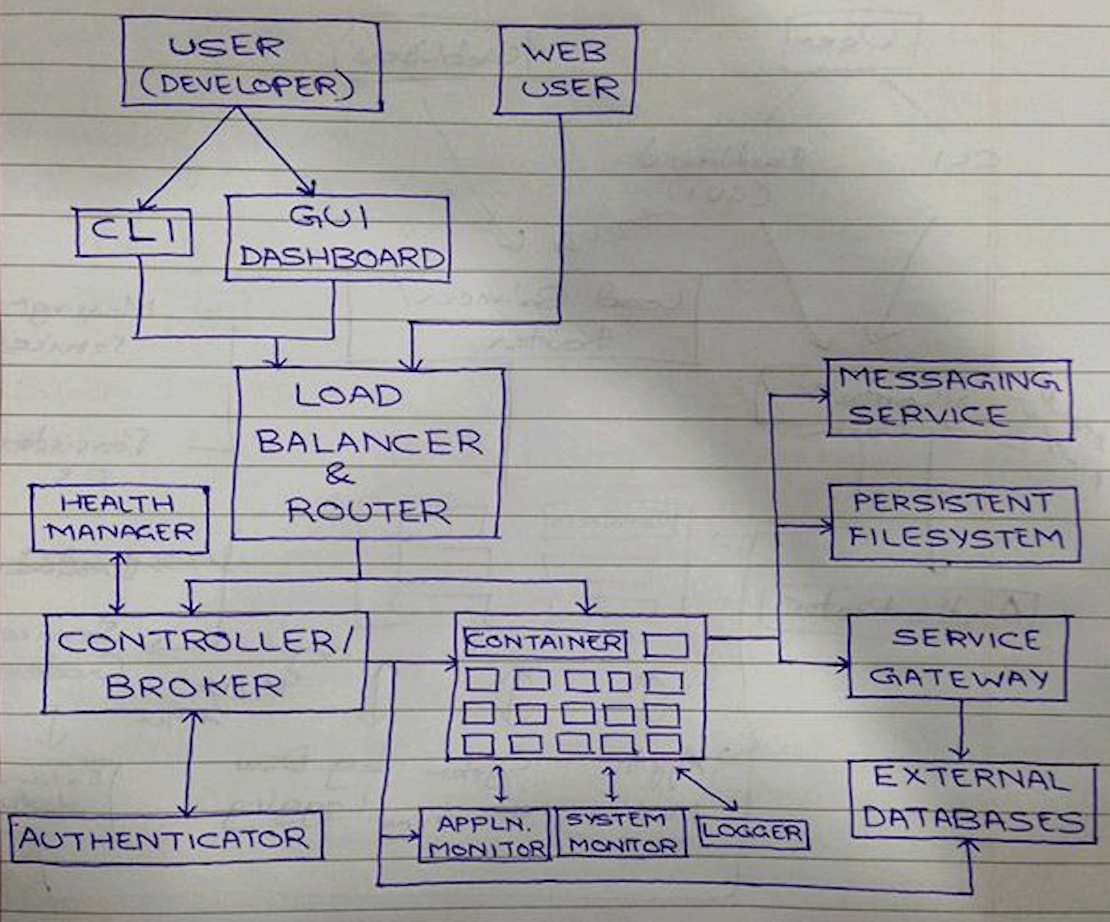
\includegraphics[width=0.8\textwidth]{flow.png}
  \caption{\label{ordering}Ordering}
  \end{figure}  

  \section{Evaluation}
  
  \subsection{Questions}
  \begin{enumerate}
	  
	  \item Performance:
	  \begin{enumerate}
	  \item Ability to honor SLAs or resource guarantees under heavy load
	  \item Efficiency of resource pooling
	  \item Rapid Elasticity? Speed of provisioning(during first instantiation as well as during sudden increase in demand)
	  \item Inter container communication speed/ delay/ latency
	  \item Difference in time required to handle HTTP requests when using containers in our cloud and in case they were running on a single machine
	  \item Speed up due to load balancer
	  \item Overhead of applications that help in the running of the cloud(i.e. due to the components mentioned above)
	  \item Mean time to respond after a failure
	  \end{enumerate}
	  
	  \item Correctness: We plan to use robust protocols like TCP for communication so there's no question of errors in messages creeping in. However, it could be the case that if a task is distributed amongst containers and the result from all of them is summed up to give the final output incorrect results may come up if there are problems in the way tasks are split up into containers and then retrieved or because of errors in synchronization. Whether or not such problems can come up will depend on our design which is yet to fully complete.
	  
	  \item Tradeoffs: There's an inherent tradeoff we make during provisioning. Whether or not to keep free memory to allow running applications to scale up faster on the same machine or cram as many containers on the same physical machines as possible to make best use of running machines.
  \end{enumerate}
  
  \subsection{Setup}
  
  Functions/ modules will be inserted at appropriate places to collect statistics about the fore-mentioned parameters. For example, to measure the delay in servicing HTTP requests, we will track time in the controller to see how much time was spent between the request from a particular IP arrived and when it was serviced(ie. responses were sent). Test java applications will be written and performance will be checked. Nodes will be deliberately failed in order to see the effectiveness of replication and check for disruption. Automated requests will be made for the web applications to see the effectiveness of horizontal scaling.
  
  \setlength{\tabcolsep}{12pt}
  \section{Timeline}
  \begin{tabular}{ll}
  Week 1 & Enrich and complete the described design and arrange machines \\
  Week 2 & Install linux, docker, openstack and other tools on all machines \\
  Week 3\&4 & Implement the controller, execution agent, messaging,\\
  & router and service abstraction components \\
  Week 5 & Make the front end webpage/ dashboard, command line tool, install \\
  & frameworks for the environments we want to provide to applications \\
  Week 6 & Carry out evaluation \\
  \end{tabular} 
 

\end{document}

